\documentclass{article}
\usepackage{amsmath}
\usepackage{amssymb}
\usepackage{tikz}
\usetikzlibrary{decorations.pathreplacing}

\begin{document}

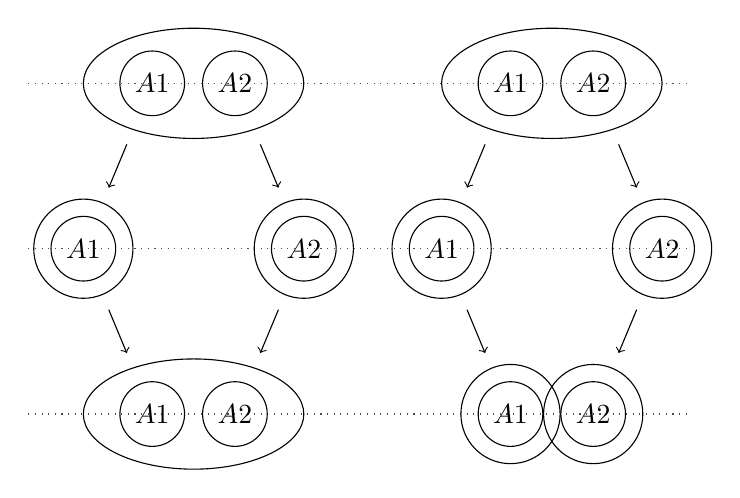
\begin{tikzpicture}[scale =0.7]


\node[shape=circle,draw=black] (s1) at (-0.75,0) {$A1$};
\node[shape=circle,draw=black] (s2) at (-2,3){$A1$};
\node[shape=circle,draw=black] (s3) at (-0.75,6){$A1$};

\node[shape=circle,draw=black] (s4) at (0.75,0){$A2$};
\node[shape=circle,draw=black] (s5) at (2,3){$A2$};
\node[shape=circle,draw=black] (s6) at (0.75,6){$A2$};

\draw (0,0) ellipse (2 and 1);

\draw[](2,3)circle (0.9);
\draw[](-2,3)circle (0.9);

\draw (0,6) ellipse (2 and 1);
    
 \path [->, shorten >=12pt,shorten <=12pt] (s2) edge node[left] {} (s1);
 \path [->, shorten >=12pt,shorten <=12pt] (s3) edge node[left] {} (s2);
 
 \path [->, shorten >=12pt,shorten <=12pt] (s5) edge node[left] {} (s4);
 \path [->, shorten >=12pt,shorten <=12pt] (s6) edge node[left] {} (s5);



\node[shape=circle,draw=black] (s7) at (-0.75 + 6.5,0) {$A1$};
\node[shape=circle,draw=black] (s8) at (-2 + 6.5,3){$A1$};
\node[shape=circle,draw=black] (s9) at (-0.75 + 6.5,6){$A1$};

\node[shape=circle,draw=black] (s10) at (0.75 + 6.5,0){$A2$};
\node[shape=circle,draw=black] (s11) at (2 + 6.5,3){$A2$};
\node[shape=circle,draw=black] (s12) at (0.75 + 6.5,6){$A2$};


\draw[](2 + 6.5,3)circle (0.9);
\draw[](-2 + 6.5,3)circle (0.9);

\draw (0 + 6.5,6) ellipse (2 and 1);

\draw[](-0.75 + 6.5,0)circle (0.9);
\draw[](0.75 + 6.5,0) circle (0.9);
    
 \path [->, shorten >=12pt,shorten <=12pt] (s8) edge node[left] {} (s7);
 \path [->, shorten >=12pt,shorten <=12pt] (s9) edge node[left] {} (s8);
 
 \path [->, shorten >=12pt,shorten <=12pt] (s11) edge node[left] {} (s10);
 \path [->, shorten >=12pt,shorten <=12pt] (s12) edge node[left] {} (s11);

 \draw [draw=black, opacity=0.7, dotted] ( -3 , 6 ) -- ( 9 , 6 );
 \draw [draw=black, opacity=0.7, dotted] ( -3 , 3 ) -- ( 9 , 3 );
 \draw [draw=black, opacity=0.7, dotted] ( -3 , 0 ) -- ( 9 , 0 );

\end{tikzpicture}

\end{document}